\documentclass[fleqn]{beamer}

\usepackage[british]{babel}
\usepackage{graphicx,ru,url}
\usepackage{amsmath}
% Use Times for math font and text font.
\RequirePackage[T1]{fontenc}
%\RequirePackage{txfonts}
% bold math must be loaded after Times font
\usepackage{bm}
\usepackage{booktabs} % nice rules (thick lines) for tables
\usepackage{microtype} % improves typography for PDF
\usepackage{xcolor} % Allows colors in fonts
\usepackage{tikz} % Allows creation of tikz pictures
\usepackage{verbatim}
\usetikzlibrary{arrows,shapes,snakes}
\usepackage{hyperref}
\usepackage{subcaption}
\renewcommand{\vec}[1]{\ensuremath{\bm{#1}}}

% The title of the presentation:
%  - first a short version which is visible at the bottom of each slide;
%  - second the full title shown on the title slide;
\title[SPH Demo]{
    Spatial Homogenization using SPH Factors}

% Optional: a subtitle to be displayed on the title slide
%\subtitle{Show where you're from}

% The author(s) of the presentation:
%  - again first a short version to be displayed at the bottom;
%  - next the full list of authors, which may include contact information;
\author[Reed]{
    Richard L. Reed}

% The institute:
%  - to start the name of the university as displayed on the top of each slide
%    this can be adjusted such that you can also create a Dutch version
%  - next the institute information as displayed on the title slide
\institute[Kansas State University]{
    Mechanical and Nuclear Engineering \\
    Kansas State University}

% Add a date and possibly the name of the event to the slides
%  - again first a short version to be shown at the bottom of each slide
%  - second the full date and event name for the title slide
\date[CORPS-G Meeting]{
    CORPS-G Meeting \\
    2019/1/25}

\begin{document}

    \begin{frame}
        \titlepage
    \end{frame}

    \begin{frame}
        \frametitle{Outline}
        \begin{block}{Presentation Outline}
            \begin{itemize}
                \item Multigroup Framework
                \item SPH factors
                \item Example
            \end{itemize}
        \end{block}
    \end{frame}

    \section{Multigroup Framework}

    \begin{frame}
        \frametitle{The Neutron Transport Equation}
        \centering
        \begin{block}{}
            When modeling a nuclear reactor, we are ultimately trying to solve this equation as accurately as possible.
            \begin{align*}
                \vec{\Omega}\cdot&\nabla\psi(\vec{r},E,\vec{\Omega})
                +\Sigma_t(\vec{r},E)\psi(\vec{r},E,\vec{\Omega})\\
                &=\int_{4\pi}\int_0^\infty\Sigma_s(\vec{r},E\leftarrow E',\vec{\Omega}\cdot\vec{\Omega}')\psi(\vec{r},E',\vec{\Omega'})dE'd\vec{\Omega}'\\
                &+\frac{\chi(\vec{r},E)}{4\pi k_{\text{eff}}}\int_0^\infty\nu\Sigma_f(\vec{r},E')\phi(\vec{r},E')dE'
            \end{align*}
            However, even if it were solvable directly, it cannot reasonably fit onto a computer.
            We thus turn to approximations.
        \end{block}
    \end{frame}

    \begin{frame}
        \centering
        \frametitle{The transport equation is solved in stages}
        \tikzstyle{decision} = [diamond, draw, fill=blue!20,
            text width=4.5em, text badly centered, node distance=3cm, inner sep=0pt]
        \tikzstyle{block} = [rectangle, draw, fill=blue!20,
            text width=13em, text centered, rounded corners, minimum height=4em]
        \tikzstyle{line} = [draw, -latex']
        \tikzstyle{cloud} = [draw, ellipse,fill=red!20, node distance=5cm,
            text width=6em, text centered, minimum height=2em]
        \begin{tikzpicture}[node distance = 2cm, auto]
            % Place nodes
            \node [block] (init) {Isotopic cross sections};
            \node [block, below of=init] (identify) {Self shielding calculations \\ $>$10000 groups};
            \node [cloud, right of=identify] (cond1) {Infinite, homogeneous medium};
            \node [block, below of=identify] (evaluate) {Lattice calculations \\ $\approx$100 groups};
            \node [cloud, right of=evaluate] (cond2) {Multigroup};
            \node [block, below of=evaluate] (stop) {Nodal core model \\ $\approx$7 groups};
            % Draw edges
            \path [line] (init) -- (identify);
            \path [line] (cond1) -- (identify);
            \path [line] (identify) -- (evaluate);
            \path [line] (cond2) -- (evaluate);
            \path [line] (evaluate) -- (stop);
        \end{tikzpicture}
    \end{frame}

    \begin{frame}
        \frametitle{The cross sections are highly energy dependent}
        \centering
        Total cross sections of H-1 and U-238
        \begin{figure}[htb]
            \begin{subfigure}{0.5\textwidth}
                \centering
                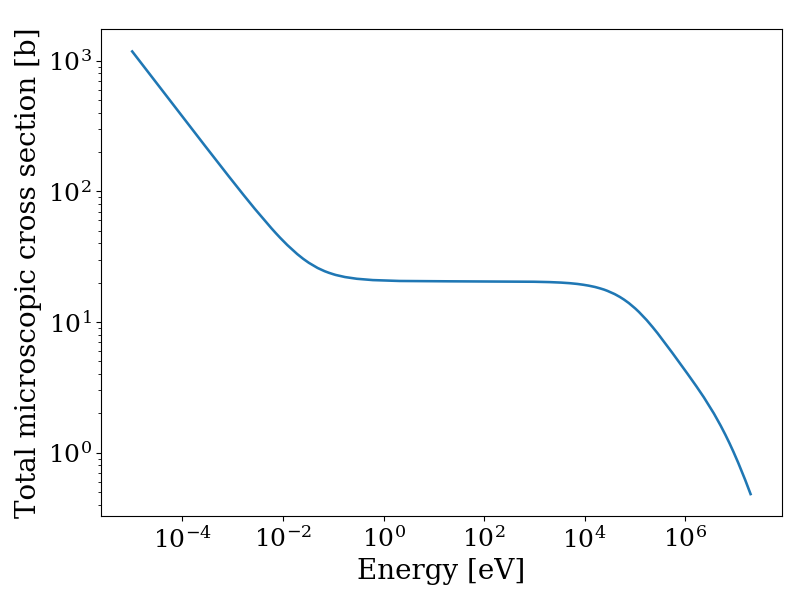
\includegraphics[totalheight=0.45\textheight]{figures/h1}
                \label{fig:XS_H1}
            \end{subfigure}%
            \begin{subfigure}{0.5\textwidth}
                \centering
                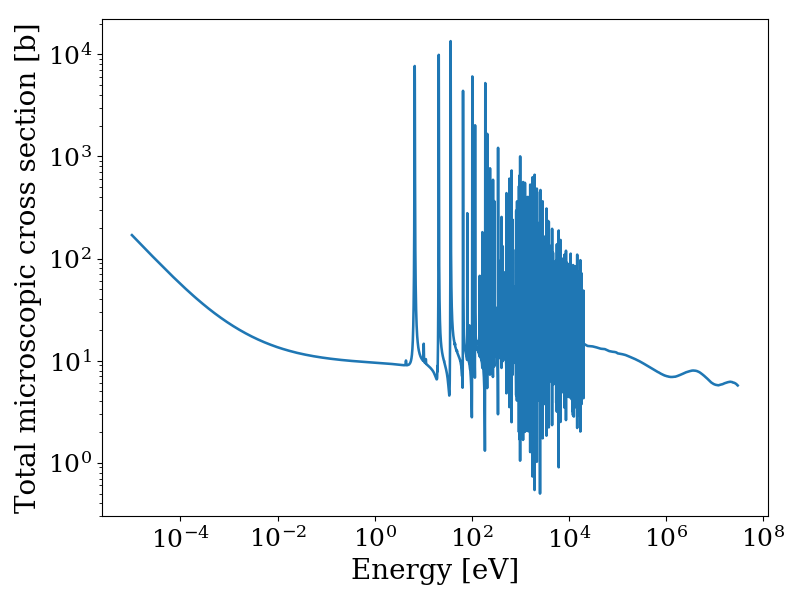
\includegraphics[totalheight=0.45\textheight]{figures/u238}
                \label{fig:XS_U238}
            \end{subfigure}%
        \end{figure}
    \end{frame}

    \begin{frame}
        \frametitle{Average over energy to find the multigroup cross section}

        \begin{block}{We want to preserve the reaction rate}
            \begin{align*}
                \bar{R}_{g}(\vec{r}) &= \frac{\int_{E_1}^{E_2}\Sigma(\vec{r}, E)\phi(\vec{r},E)dE}{\int_{E_1}^{E_2}dE}\\
                \bar{R}_{g}(\vec{r}) &= \bar{\Sigma}_{g}(\vec{r})\frac{\int_{E_1}^{E_2}\phi(\vec{r},E)dE}{\int_{E_1}^{E_2}dE}\\
                \bar{R}_{g}(\vec{r}) &= \bar{\Sigma}_{g}(\vec{r})\bar{\phi}_{g}(\vec{r})
            \end{align*}
        \end{block}

        \begin{block}{The Multigroup cross section is defined}
            \begin{equation*}
                \bar{\Sigma}_g(\vec{r}) = \frac{\int_{E_1}^{E_2}\Sigma(\vec{r},E)\phi(\vec{r},E)dE}{\int_{E_1}^{E_2}\phi(\vec{r},E)dE}
            \end{equation*}
        \end{block}
    \end{frame}

    \begin{frame}
        \frametitle{The Multigroup Equation}
        \centering
        \begin{block}{Substitute the definition into the neutron transport equation}
            \begin{align*}
                \vec{\Omega}\cdot\nabla\psi_g(\vec{r},\vec{\Omega})
                &+\Sigma_{t,g}(\vec{r})\psi_g(\vec{r},\vec{\Omega})\\
                &=\int_{4\pi}\sum_{g'=1}^{N_g}\Sigma_{s,g\leftarrow g'}(\vec{r},\vec{\Omega}\cdot\vec{\Omega}')\psi_{g'}(\vec{r},\vec{\Omega'})d\vec{\Omega}'\\
                &+\frac{\chi_g(\vec{r})}{4\pi k_{\text{eff}}}\sum_{g'=1}^{N_g}\nu\Sigma_{f,g'}(\vec{r})\phi_{g'}(\vec{r})
            \end{align*}
            Notice that the solution was required to solve for the cross sections.
            Also, we still have to treat space and angle!
        \end{block}
    \end{frame}

    \section{SPH factors} % new section title

    \begin{frame}
        \frametitle{The flux looks different at each stage of modeling}
        \begin{center}
            \begin{figure}[htb]
                \begin{subfigure}{0.24\textwidth}
                    \centering
                    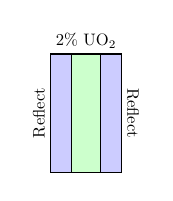
\begin{tikzpicture}[scale=0.6, every node/.style={scale=0.6}]
                        \foreach \x in {0}
                        \filldraw[xshift=\x cm, fill=green!20!white, draw=black] (0.45,0) rectangle (1.05,2.5);
                        \foreach \x in {0}
                        \filldraw[xshift=\x cm, fill=blue!20!white, draw=black] (0,0) rectangle (0.45,2.5);
                        \foreach \x in {0}
                        \filldraw[xshift=\x cm, fill=blue!20!white, draw=black] (1.05,0) rectangle (1.5,2.5);
                        \draw[xshift=0.75cm,yshift=2.5cm] node[above] {{2\% UO$_2$}};
                        \draw[xshift=1.5cm,yshift=1.25cm] node[right] {\rotatebox{-90}{Reflect}};
                        \draw[yshift=1.25cm] node[left] {\rotatebox{90}{Reflect}};
                    \end{tikzpicture}
                \end{subfigure}
                \begin{subfigure}{0.24\textwidth}
                    \centering
                    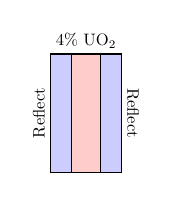
\begin{tikzpicture}[scale=0.6, every node/.style={scale=0.6}]
                        \foreach \x in {0}
                        \filldraw[xshift=\x cm, fill=red!20!white, draw=black] (0.45,0) rectangle (1.05,2.5);
                        \foreach \x in {0}
                        \filldraw[xshift=\x cm, fill=blue!20!white, draw=black] (0,0) rectangle (0.45,2.5);
                        \foreach \x in {0}
                        \filldraw[xshift=\x cm, fill=blue!20!white, draw=black] (1.05,0) rectangle (1.5,2.5);
                        \draw[xshift=0.75cm,yshift=2.5cm] node[above] {{4\% UO$_2$}};
                        \draw[xshift=1.5cm,yshift=1.25cm] node[right] {\rotatebox{-90}{Reflect}};
                        \draw[yshift=1.25cm] node[left] {\rotatebox{90}{Reflect}};
                    \end{tikzpicture}
                \end{subfigure}
                \begin{subfigure}{0.24\textwidth}
                    \centering
                    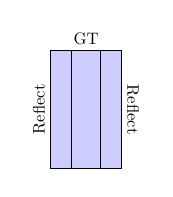
\begin{tikzpicture}[scale=0.6, every node/.style={scale=0.6}]
                        \foreach \x in {0}
                        \filldraw[xshift=\x cm, fill=blue!20!white, draw=black] (0.45,0) rectangle (1.05,2.5);
                        \foreach \x in {0}
                        \filldraw[xshift=\x cm, fill=blue!20!white, draw=black] (0,0) rectangle (0.45,2.5);
                        \foreach \x in {0}
                        \filldraw[xshift=\x cm, fill=blue!20!white, draw=black] (1.05,0) rectangle (1.5,2.5);
                        \draw[xshift=0.75cm,yshift=2.5cm] node[above] {{GT}};
                        \draw[xshift=1.5cm,yshift=1.25cm] node[right] {\rotatebox{-90}{Reflect}};
                        \draw[yshift=1.25cm] node[left] {\rotatebox{90}{Reflect}};
                    \end{tikzpicture}
                \end{subfigure}
                \begin{subfigure}{0.24\textwidth}
                    \centering
                    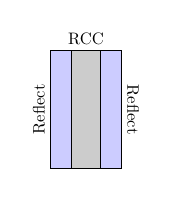
\begin{tikzpicture}[scale=0.6, every node/.style={scale=0.6}]
                        \foreach \x in {0}
                        \filldraw[xshift=\x cm, fill=black!20!white, draw=black] (0.45,0) rectangle (1.05,2.5);
                        \foreach \x in {0}
                        \filldraw[xshift=\x cm, fill=blue!20!white, draw=black] (0,0) rectangle (0.45,2.5);
                        \foreach \x in {0}
                        \filldraw[xshift=\x cm, fill=blue!20!white, draw=black] (1.05,0) rectangle (1.5,2.5);
                        \draw[xshift=0.75cm,yshift=2.5cm] node[above] {{RCC}};
                        \draw[xshift=1.5cm,yshift=1.25cm] node[right] {\rotatebox{-90}{Reflect}};
                        \draw[yshift=1.25cm] node[left] {\rotatebox{90}{Reflect}};
                    \end{tikzpicture}
                \end{subfigure}
            \end{figure}
        \end{center}
        \begin{center}
            \begin{figure} % Here you can use any figure
                \begin{subfigure}{0.46\textwidth}
                    \centering
                    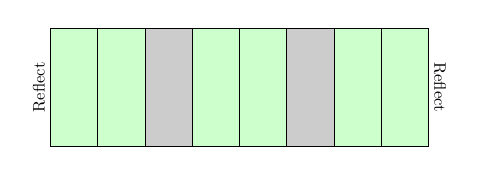
\begin{tikzpicture}[scale=0.6, every node/.style={scale=0.6}]
                        \foreach \x in {0,1,3,4,6,7}
                        \filldraw[xshift=\x cm, fill=green!20!white, draw=black] (0,0) rectangle (1,2.5);
                        \foreach \x in {2,5}
                        \filldraw[xshift=\x cm, fill=black!20!white, draw=black] (0,0) rectangle (1,2.5);
                        \draw[xshift=8cm,yshift=1.25cm] node[right] {\rotatebox{-90}{Reflect}};
                        \draw[yshift=1.25cm] node[left] {\rotatebox{90}{Reflect}};
                    \end{tikzpicture}
                \end{subfigure}
                \hfill
                \begin{subfigure}{0.46\textwidth}
                    \centering
                    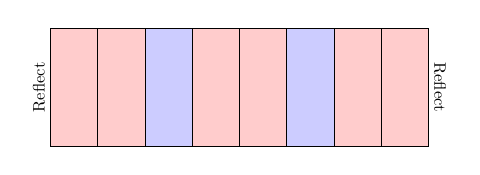
\begin{tikzpicture}[scale=0.6, every node/.style={scale=0.6}]
                        \foreach \x in {0,1,3,4,6,7}
                        \filldraw[xshift=\x cm, fill=red!20!white, draw=black] (0,0) rectangle (1,2.5);
                        \foreach \x in {2,5}
                        \filldraw[xshift=\x cm, fill=blue!20!white, draw=black] (0,0) rectangle (1,2.5);
                        \draw[xshift=8cm,yshift=1.25cm] node[right] {\rotatebox{-90}{Reflect}};
                        \draw[yshift=1.25cm] node[left] {\rotatebox{90}{Reflect}};
                    \end{tikzpicture}
                \end{subfigure}
            \end{figure}
        \end{center}
        \begin{figure} % Here you can use any figure
            \centering
            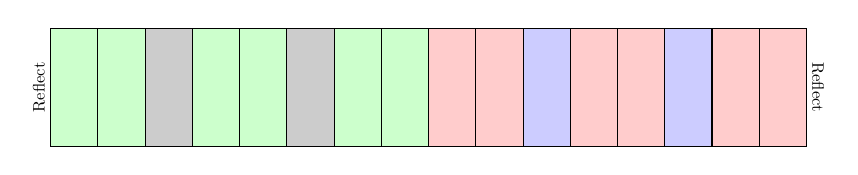
\begin{tikzpicture}[scale=0.6, every node/.style={scale=0.6}]
                \foreach \x in {0,1,3,4,6,7}
                \filldraw[xshift=\x cm, fill=green!20!white, draw=black] (0,0) rectangle (1,2.5);
                \foreach \x in {2,5}
                \filldraw[xshift=\x cm, fill=black!20!white, draw=black] (0,0) rectangle (1,2.5);
                \foreach \x in {8,9,11,12,14,15}
                \filldraw[xshift=\x cm, fill=red!20!white, draw=black] (0,0) rectangle (1,2.5);
                \foreach \x in {10,13}
                \filldraw[xshift=\x cm, fill=blue!20!white, draw=black] (0,0) rectangle (1,2.5);
                \draw[xshift=16cm,yshift=1.25cm] node[right] {\rotatebox{-90}{Reflect}};
                \draw[yshift=1.25cm] node[left] {\rotatebox{90}{Reflect}};
            \end{tikzpicture}
        \end{figure}
    \end{frame}

    \begin{frame}
        \frametitle{Spatial homogenization}
        \centering
        \begin{block}{Consider only one energy group}
            \begin{equation*}
                R(x) = \Sigma(x)\phi(x)
            \end{equation*}
        \end{block}
        \begin{block}{Spatially averaged reaction rate}
            \begin{equation*}
                \bar{R} = \frac{\int\Sigma(x)\phi(x)dx}{\int dx}=\bar{\Sigma}\frac{\int\phi(x)dx}{\int dx}=\bar{\Sigma}\bar{\phi}
            \end{equation*}
        \end{block}
        \begin{block}{The flux is different for the homogenized case}
            \begin{equation*}
                \bar{R}^* = \frac{\int\Sigma(x)\phi^*(x)dx}{\int dx}=\bar{\Sigma}^*\frac{\int\phi^*(x)dx}{\int dx}=\bar{\Sigma}^*\bar{\phi}^*
            \end{equation*}
        \end{block}
    \end{frame}

    \begin{frame}
        \frametitle{Spatial homogenization}
        \centering
        \begin{block}{Equate the reaction rates for and aft homogenization}
            \begin{equation*}
                \bar{\Sigma}^*\bar{\phi}^* = \bar{R}^* = \bar{R} = \bar{\Sigma}\bar{\phi}
            \end{equation*}
        \end{block}
        \begin{block}{Thus the cross sections for the homogenized case are different}
            \begin{equation*}
                \bar{\Sigma}^* = \bar{\Sigma}\frac{\bar{\phi}}{\bar{\phi}^*} = \bar{\Sigma}\mu
                \quad\text{where}\quad
                \mu=\frac{\bar{\phi}}{\bar{\phi}^*}
            \end{equation*}
        \end{block}
    \end{frame}

    \begin{frame}
        \frametitle{The SPH proceedure}
        \begin{block}{Thus the cross sections for the homogenized case are different}
            \begin{equation*}
                \bar{\Sigma}^\text{homog} = \bar{\Sigma}^\text{ref}\frac{\bar{\phi}^\text{ref}}{\bar{\phi}^\text{homog}} = \bar{\Sigma}^\text{ref}\mu
                \quad\text{where}\quad
                \mu=\frac{\bar{\phi}}{\bar{\phi}^*}
            \end{equation*}
        \end{block}
        \begin{block}{Simple procedure to preserve reaction rates}
            \begin{enumerate}
                \item Compute the reference (spatially fine) solution
                \item Homogenize the cross sections
                \item Compute the homogenized solution
                \item Compute $\mu$, the SPH factors
                \item Update the homogenized cross sections with new $\mu$
                \item Return to step 3 until converged $\mu$ values
            \end{enumerate}
        \end{block}
    \end{frame}

    \section{Example}
    \begin{frame}
        \frametitle{Comparison for absorption rate}
        \centering
        \begin{figure}
            \centering
            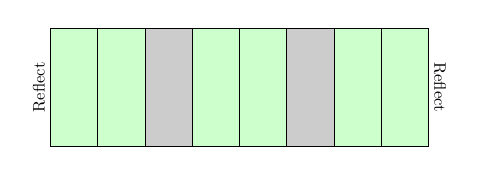
\begin{tikzpicture}[scale=0.6, every node/.style={scale=0.6}]
                \foreach \x in {0,1,3,4,6,7}
                \filldraw[xshift=\x cm, fill=green!20!white, draw=black] (0,0) rectangle (1,2.5);
                \foreach \x in {2,5}
                \filldraw[xshift=\x cm, fill=black!20!white, draw=black] (0,0) rectangle (1,2.5);
                \draw[xshift=8cm,yshift=1.25cm] node[right] {\rotatebox{-90}{Reflect}};
                \draw[yshift=1.25cm] node[left] {\rotatebox{90}{Reflect}};
            \end{tikzpicture}
        \end{figure}
        \begin{figure}[htb]
            \begin{subfigure}{0.5\textwidth}
                \centering
                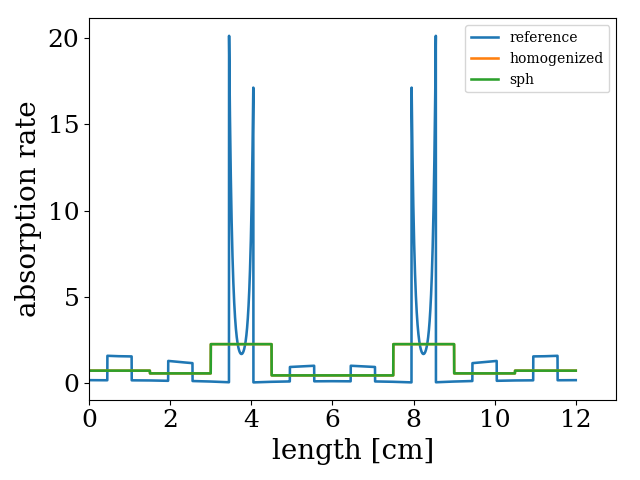
\includegraphics[totalheight=0.5\textheight]{figures/abs_rate_assay1}
                \label{fig:XS_H1}
            \end{subfigure}%
            \begin{subfigure}{0.5\textwidth}
                \centering
                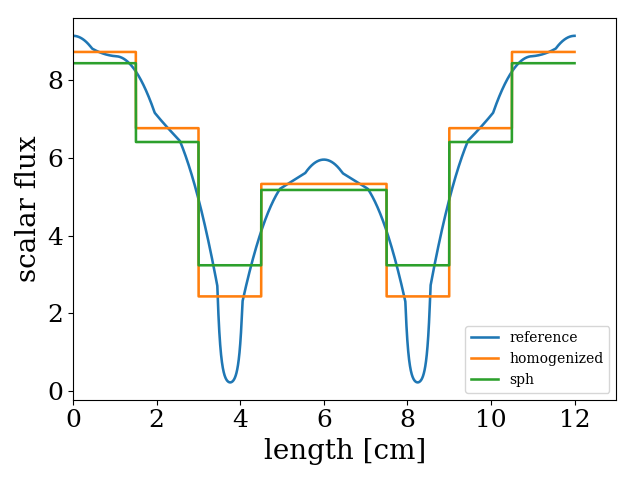
\includegraphics[totalheight=0.5\textheight]{figures/scalar_flux_assay1}
                \label{fig:XS_U238}
            \end{subfigure}%
        \end{figure}
    \end{frame}

    \begin{frame}
        \frametitle{Comparison for absorption rate}
        \centering
        \begin{figure}
            \centering
            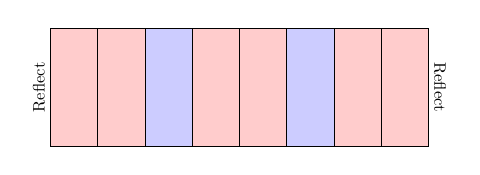
\begin{tikzpicture}[scale=0.6, every node/.style={scale=0.6}]
                \foreach \x in {0,1,3,4,6,7}
                \filldraw[xshift=\x cm, fill=red!20!white, draw=black] (0,0) rectangle (1,2.5);
                \foreach \x in {2,5}
                \filldraw[xshift=\x cm, fill=blue!20!white, draw=black] (0,0) rectangle (1,2.5);
                \draw[xshift=8cm,yshift=1.25cm] node[right] {\rotatebox{-90}{Reflect}};
                \draw[yshift=1.25cm] node[left] {\rotatebox{90}{Reflect}};
            \end{tikzpicture}
        \end{figure}
        \begin{figure}[htb]
            \begin{subfigure}{0.5\textwidth}
                \centering
                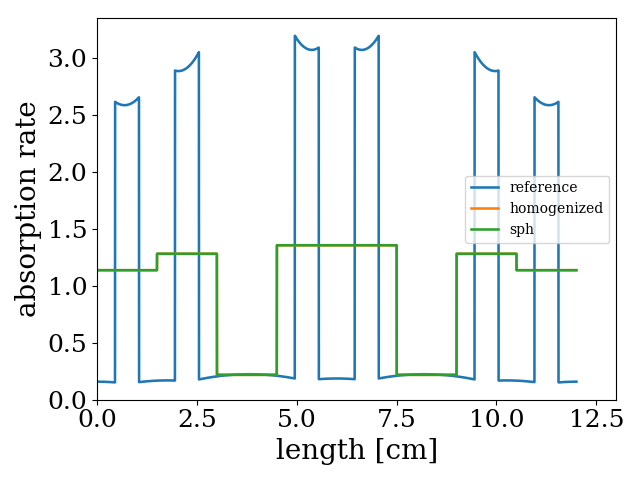
\includegraphics[totalheight=0.5\textheight]{figures/abs_rate_assay2}
                \label{fig:XS_H1}
            \end{subfigure}%
            \begin{subfigure}{0.5\textwidth}
                \centering
                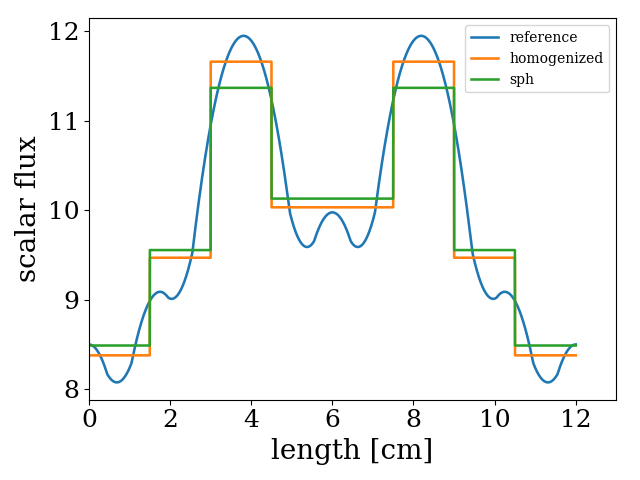
\includegraphics[totalheight=0.5\textheight]{figures/scalar_flux_assay2}
                \label{fig:XS_U238}
            \end{subfigure}%
        \end{figure}
    \end{frame}

    \begin{frame}
        \frametitle{Comparison for absorption rate}
        \centering
        \begin{figure} % Here you can use any figure
            \centering
            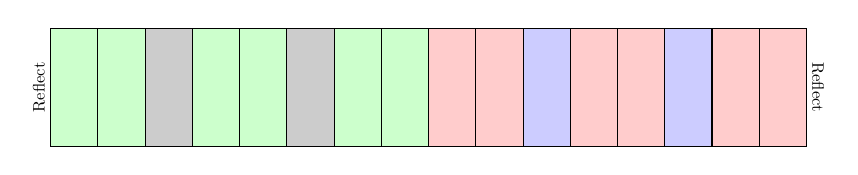
\begin{tikzpicture}[scale=0.6, every node/.style={scale=0.6}]
                \foreach \x in {0,1,3,4,6,7}
                \filldraw[xshift=\x cm, fill=green!20!white, draw=black] (0,0) rectangle (1,2.5);
                \foreach \x in {2,5}
                \filldraw[xshift=\x cm, fill=black!20!white, draw=black] (0,0) rectangle (1,2.5);
                \foreach \x in {8,9,11,12,14,15}
                \filldraw[xshift=\x cm, fill=red!20!white, draw=black] (0,0) rectangle (1,2.5);
                \foreach \x in {10,13}
                \filldraw[xshift=\x cm, fill=blue!20!white, draw=black] (0,0) rectangle (1,2.5);
                \draw[xshift=16cm,yshift=1.25cm] node[right] {\rotatebox{-90}{Reflect}};
                \draw[yshift=1.25cm] node[left] {\rotatebox{90}{Reflect}};
            \end{tikzpicture}
        \end{figure}
        \begin{figure}[htb]
            \begin{subfigure}{0.5\textwidth}
                \centering
                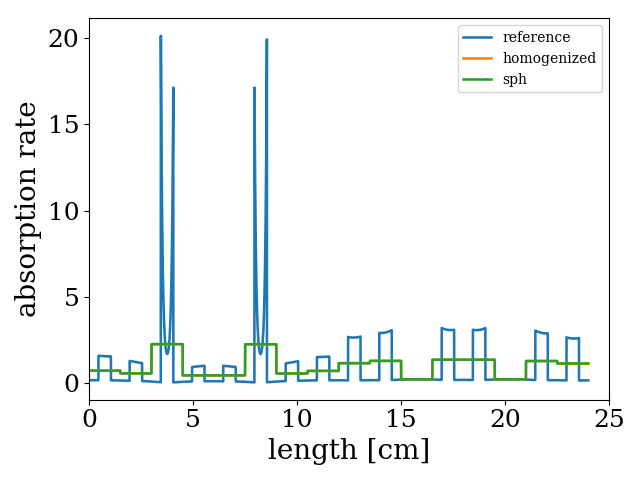
\includegraphics[totalheight=0.5\textheight]{figures/abs_rate}
                \label{fig:XS_H1}
            \end{subfigure}%
            \begin{subfigure}{0.5\textwidth}
                \centering
                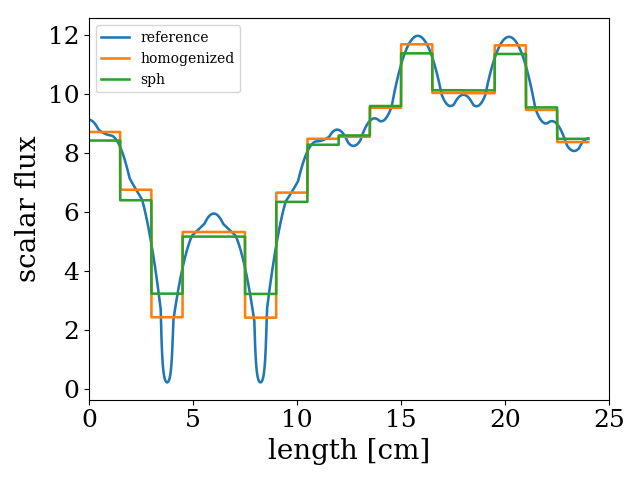
\includegraphics[totalheight=0.5\textheight]{figures/scalar_flux}
                \label{fig:XS_U238}
            \end{subfigure}%
        \end{figure}
        -0.00  -0.00 -0.00 -0.01 -0.03  0.18  0.54  0.91 \\
        -0.73 -0.26 -0.12 -0.05 -0.02 -0.01 -0.00 -0.00
    \end{frame}

\end{document}
